\section{Anatomy of the lower arm}

%Anatomy of the arm 
%	Which muscles do we measure EMG from?
%	How does the muscles relate to movement of the arm/hand?

%head
%To understand how it is possible to use EMG to control robotics or prostheses, especially robotics or prostheses which %represent the human arm, it is necessary to know the anatomy of the human arm.
% --OR-- 
This project will focus on the lower arm as the Myo armband will be used to extract information from this part of the body. The anatomy of the lower human arm will briefly be described in this section along with a description of relation between lower arm muscles and hand movements for selected gestures. \\

The human arm is designed to give humans a manoeuvrability and dexterity to coordinate and execute complicated and precise hand and finger movements with ease. Each movement happens around an axis, and each axis denotes one DOF. The arm has seven DOFs, where the arm is defined as distal to the shoulder joint and proximal to the hand. This means DOFs of the hands and fingers and translation of the shoulder are not included. Thus the DOFs included in the arm are at the shoulder; abduction and adduction, flexion and extension, medial and lateral rotation. Extension and flexion at the elbow. Pronation and supination of the lower arm and at the wrist; extension and flexion, radial and ulnar deviation. \\
The number of DOFs is defined as the number of possible input parameters to a movable mechanism, where each input controls an independent movement in one axis. Several bodies can work together in relation to each other, but the total number of DOFs will be the number of possible independent movements that can be performed between the bodies. \cite{dicker2003} \\
The great dexterity of the human arm is achieved through the use of several muscles which intertwine and make synergies to perform all the different gestures of the hand \cite{jiang2009, avella2006}. Muscles in the lower arm is arranged in layers, having an outer, middle and inner layer. These muscles are used to rotate the forearm, flex and extend the hand at the wrist as well as performing ulnar and radial deviation. The muscles control extension and flexion of the fingers at each separate joint and the movements of the thumb, so that the hand can be opened and closed. This enables movement in seven DOFs of the arm and several more at the hand and fingers. \\
The aim for this project is to translate ulnar and radial deviation along with extension and flexion of the wrist via EMG signals to achieve proportional and simultaneous control in a virtual environment. These movements are depicted in \figref{fig:wristMove}. Therefore, only these muscles will be relevant to further investigate. The number of muscles involved in radial and ulnar deviation includes several muscles in the arm. Most of these muscles extend throughout the whole forearm as most of them originates from the distal lateral surfaces of humerus or the proximal portions of radius and ulnar, and extends towards the wrist and fingers to fixate on the metacarpal bones in the wrist and through tendons fixate on the different phalanges bones of the fingers and thumb. The two most important muscles in radial/ulnar deviation are the flexor and extensor carpi ulnaris and radialis muscles. 
%Radius and ulnar deviation is depicted in \figref{fig:wrist_move}.

\begin{figure}[H] 
	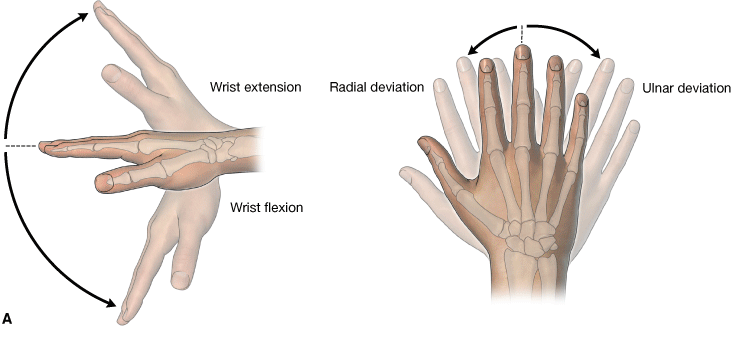
\includegraphics[width=0.5\textwidth]{figures/anatomy/flexexulradev}  %<--but is not needed.
	\caption{Flexion, extension and radial and ulnar deviation of the hand. Modified from \cite{zezo2016}}
	\label{fig:wristMove}
\end{figure}

Several more muscles in addition to those responsible for ulnar and radial deviation are involved with the flexion and extension of the wrist. Like the other muscles, the flexor and extensor muscles also extend through the whole forearm from the distal part of humerus and proximal parts of radius and ulnar to the metacarpal bones in the wrist. Many of these muscles are included in movements of both radial/ulnar deviation and flexion/extension, though flexion/extension have one muscle who is only used for flexion at the wrist, the palmaris longus muscle. This can be explained as more force is usually needed in flexion at the wrist than in extension or radial/ulnar deviation.\\
Though several of the same muscles are included in both types of movement, studies have shown that it is possible to differentiate between recorded EMG signals from these muscles when performing radial/ulnar deviation and flexion/extension at the wrist. \cite{hahne2014} In \figref{fig:ALL_THE_MUSCLES} the muscles in the forearm both involved with extension/flexion and radial/ulnar deviation is marked with boxes around the name of the muscles. 

\begin{figure}[H]
	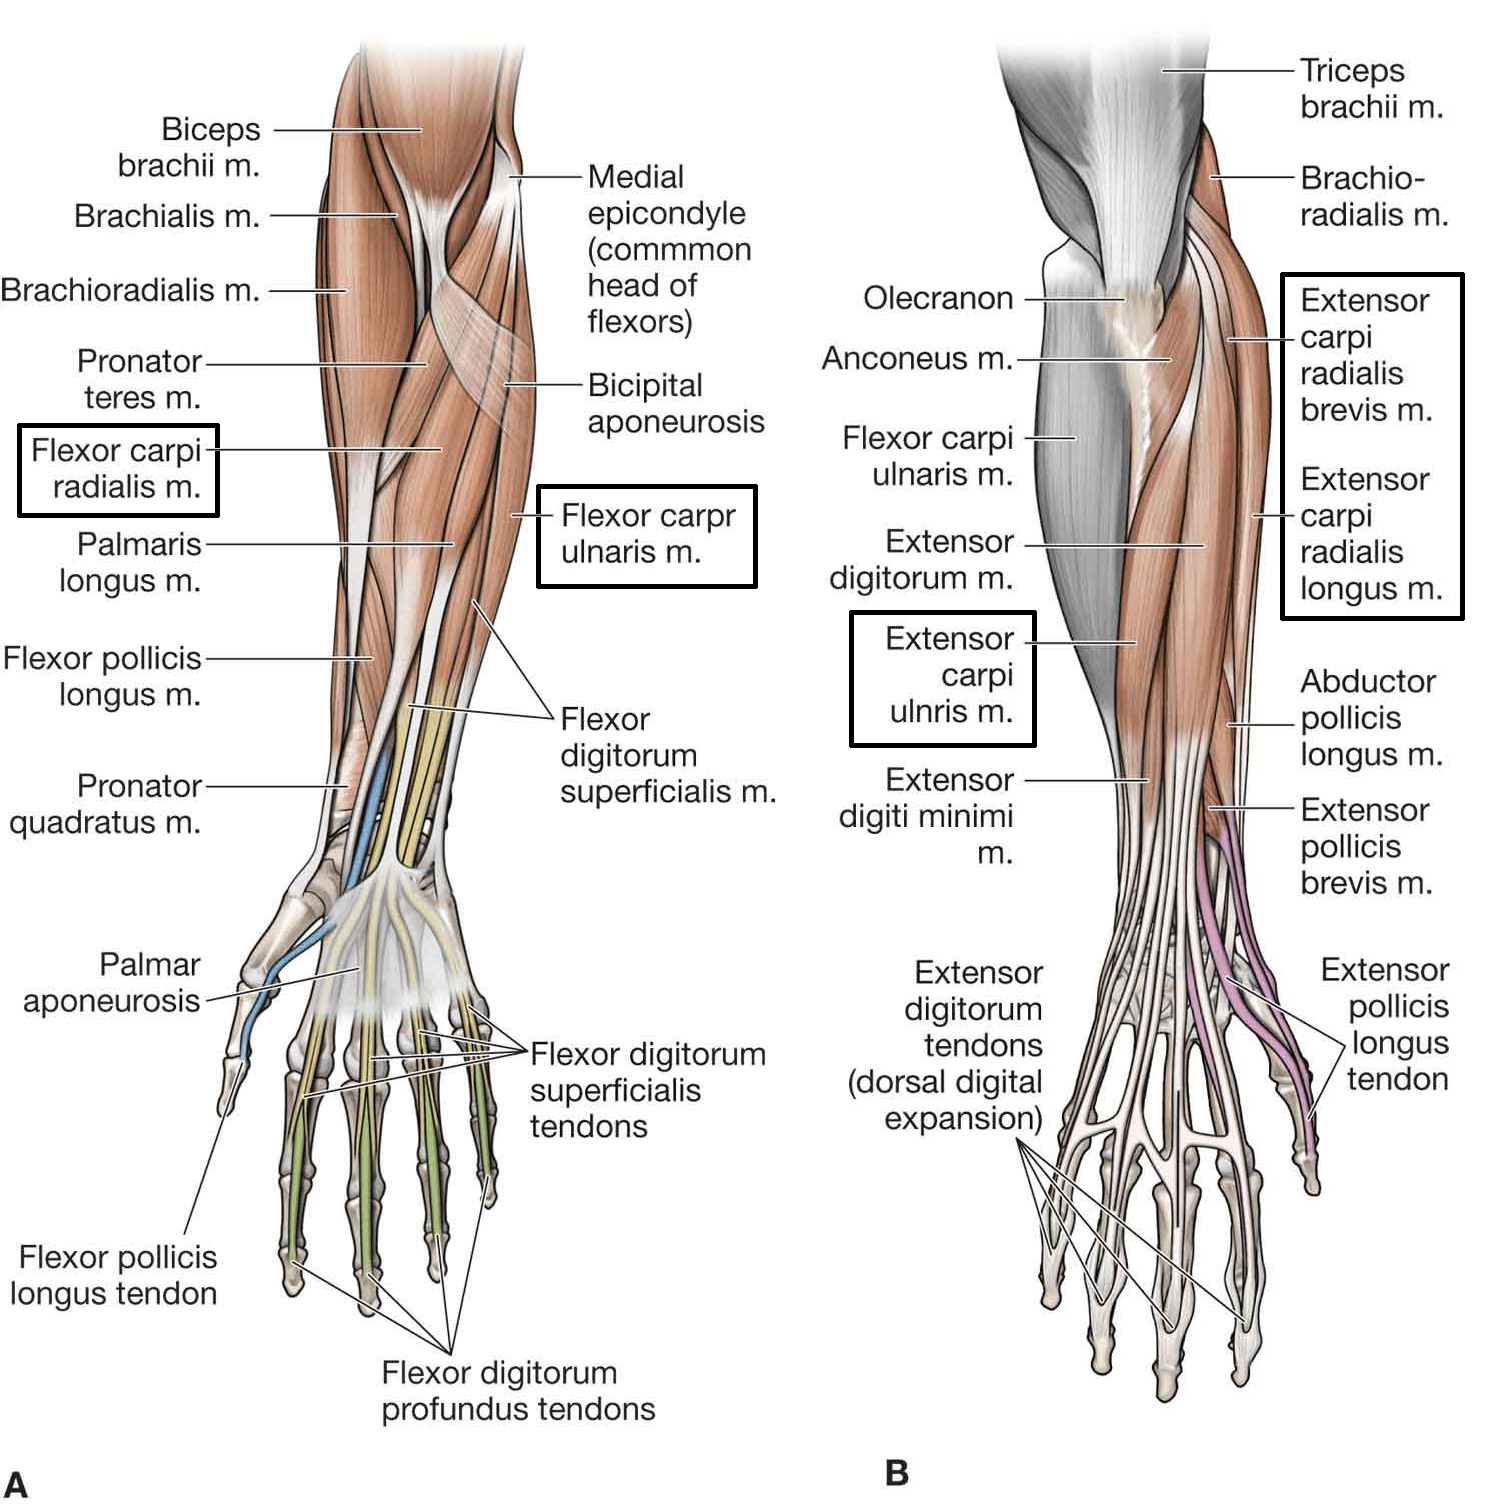
\includegraphics[width=0.7\textwidth]{figures/anatomy/all_the_muscles}  %<--but is not needed.
	\caption{\textbf{A)} anterior view of lower muscles. \textbf{B)} posterior view of lower muscles. The muscle names in the boxes are muscles which are included in both extension/flexion and ulnar/radial deviation at the wrist. Modified from \cite{zezo2016}.}
	\label{fig:ALL_THE_MUSCLES}  %<--give the figure a label, so you can reference!
\end{figure}

%Muscles involved with pronation of the wrist includes the pronator quadratus and pronator teres muscles. The pronator quadratus muscle is located near the wrist and is fixated on the distal portions of both ulna and radius, from where is forms a wide band across the gap of the two bones. The pronator teres is located near the elbow, where it originates  from the medial distal part of humerus and the medial lateral part of ulna, to reach across the anterior part of the forearm and fixate to the midlateral surface of radius. 
%There is only one muscle involved in the process of supination of the forearm, the supinator. The supinator muscle sits opposite the pronator teres muscle near the elbow, where it originates from the lateral distal part of humerus and the lateral proximal part of ulna and fixate on the anterolateral surface of radius. 
%These three are the only muscles responsible for pronation and supination of the forearm. Therein exists a problem in detecting viable EMG signals to properly detect pronation and supination gestures, since the muscles involved does not extend through the forearm as most other muscles in the forearm.

%Extension and flexion of the fingers include most of the muscles in the lower arm. Most of these muscles extend throughout the whole forearm as most of them originates from the lateral surfaces of humerus or the proximal portions of ulna and radius, and extends towards the wrist and fingers to fixate on the metacarpal bones in the wrist and through tendons fixate on the different phalanges bones of the fingers and thumb. See FIGURE \ref{fig:wrist} and \ref{fig:wristFingers} for a detailed overview of each muscles origin, insertion and action it performs. 
%
%\begin{figure}[H]
%	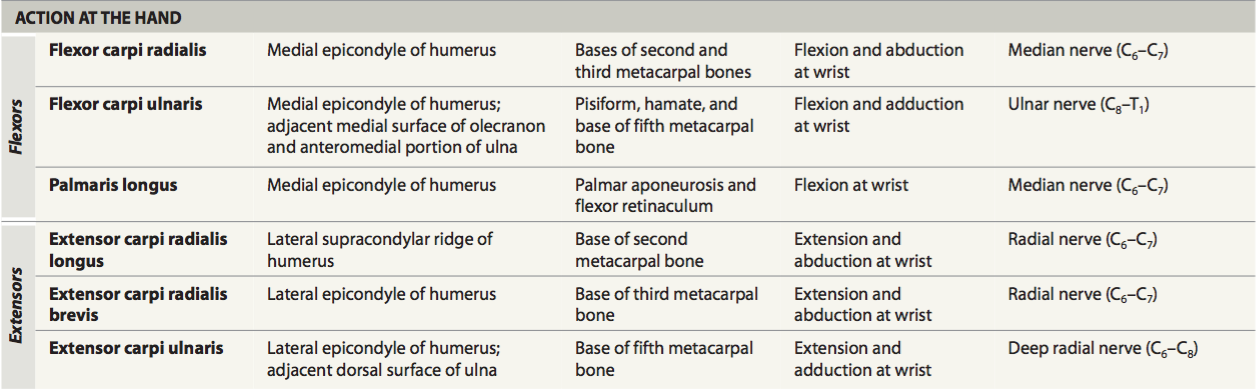
\includegraphics[width=.4\textwidth]{figures/Anatomy/wrist}  %<--but is not needed.
%	\caption{Table of the muscles in the forearm involved with movements of the wrist. \cite{martini}}
%	\label{fig:wrist}  %<--give the figure a label, so you can reference!
%\end{figure}
%
%\begin{figure}[H]                    
%	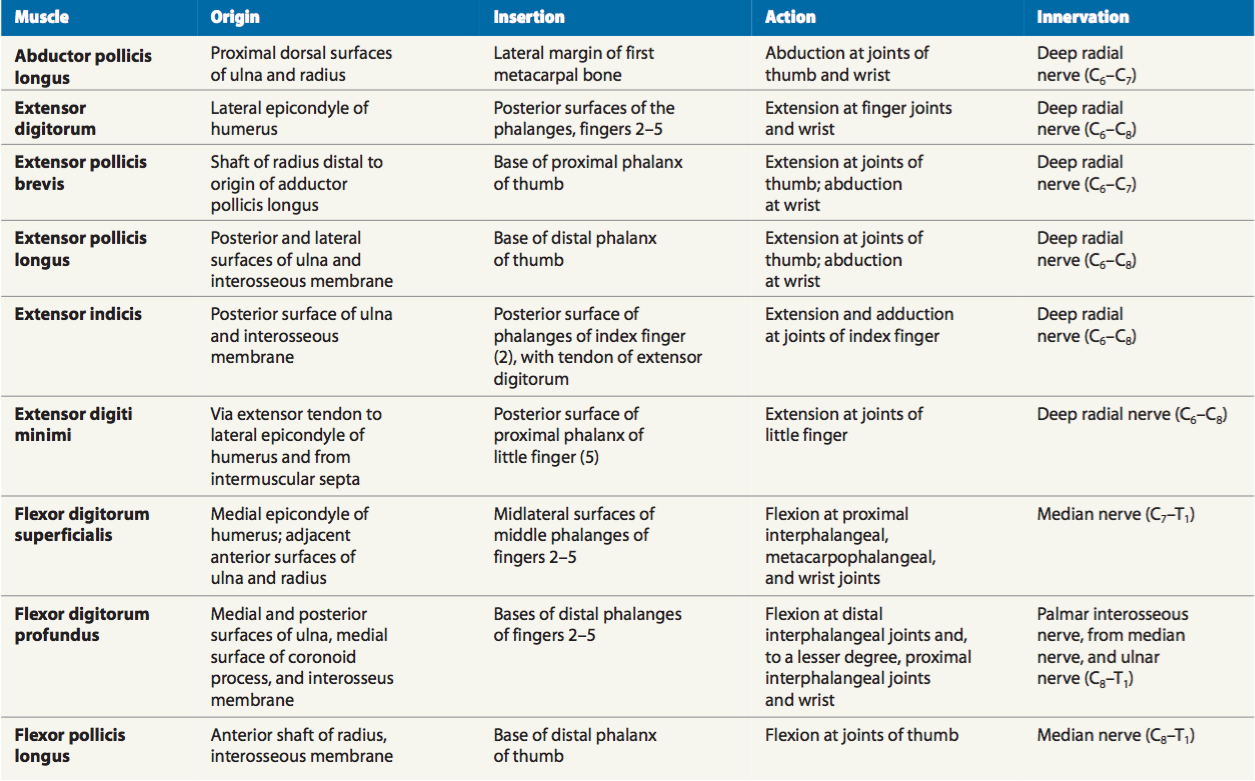
\includegraphics[width=.4\textwidth]{figures/Anatomy/wristFingers}  %<--but is not needed.
%	\caption{Tabel of muscles in the forearm involved with movements of the wrist and fingers. \cite{martini}}
%	\label{fig:wristFingers}  %<--give the figure a label, so you can reference!
%\end{figure}



%abductor pollicis longus
%extensor pollicis longus
%extensor pollicis brevis
%extensor indicis
%supinator
%anconeus
%extensor digitorum
%extensor digiti minimi
%pronator quadratus
%flexor digitorum superficialis
%brachialis
%flexor pollicis longus
%flexor digitorum profundus
%brachioradialis
%flexor carpi ulnaris
%pronator teres
%extensor carpi ulnaris
%extensor carpi radialis brevis
%extensor carpi radialis longus
%palmaris longus
%flexor carpi radialis




%tail

